\documentclass[a4paper]{article}

%% Language and font encodings
\usepackage[english]{babel}
\usepackage[utf8x]{inputenc}
\usepackage[T1]{fontenc}
\usepackage{float}
\usepackage{tikz}
\usetikzlibrary{matrix}
\usepackage{algpseudocode} 

%% Sets page size and margins
\usepackage[a4paper,top=3cm,bottom=2cm,left=3cm,right=3cm,marginparwidth=1.75cm]{geometry}
\usepackage{amsmath}
\usepackage{amsthm}
\usepackage{amssymb}

\newtheorem{theorem}{Theorem}
\newtheorem{lemma}[theorem]{Lemma}

\begin{document}
\section*{External memory mergesort}
In the external-memory model (hereafter EM model),
show how to implement the k-way merge (where $(k + 1)B \leq M$), namely, how to
simultaneously merge k sorted sequences of total length N, with an I/O cost of $O(N/B)$
where B is the block transfer size. Also, try to minimize and analyze the CPU time
cost.
\\
\\
\textbf{SOLUTION}
\\
\\
The classical external sorting algorithm, called merge-sort, consists of two phases:
\begin{enumerate}
\item \textbf{The sort phase}. M ($k*B$) element are read into the memory, sorted, and written to the
disk. This creates $n =\lceil N/M \rceil$ sorted subset of records, called runs, stored
in separate auxiliary files, numbered from 1 to n. The runs have all the same
number of elements, M, except the last.
\item \textbf{The merge phase} consists of multiple merge passes. Since we have $(k + 1)B \leq M$ then $k\leq \frac{M}{B}-1$, hence in RAM we keep k buffer of size B plus one for the output. The merge is done transferring k blocks, of size B, in main memory from the first k runs. Since each run is sorted, we keep the minimum from each run, and we store it to an other block (notice that we delete the element in the input buffer and we create a copy in the output ones). When we full fill the latter block we transfer it in external memory. At the end of a merge pass, the number of runs becomes $n=\lceil n/k \rceil$. A merge pass is repeated until
n > 1. Notice that we could add some implementation details such as a counter to keep track of how many element are still in the buffer.
\end{enumerate}
\begin{figure}[H]
\centering
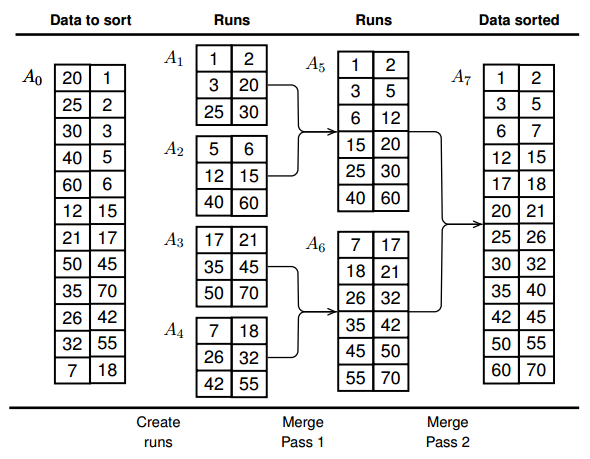
\includegraphics[scale=0.4]{kway.png}
\caption{Let us show how to sort the file $A_0$ containing 12 pages, with file and buffer pages
capacity of 2 records[\textbf{IT'S AN EXAMPLE} no need to consider the records], B = 3 and 2-merge passes.}
\end{figure}
\begin{itemize}
\item The initial sort phase creates the runs $A_1$, $A_2$, $A_3$ and $A_4$.
\item The first merge pass creates the runs $A_5$ and $A_6$ by merging $A_1$, $A_2$ and $A_3$,$A_4$.
\item The second merge pass creates the sorted data $A_7$ by merging $A_5$, $A_6$.
\end{itemize}
At each iteration of merge we read $\lceil \frac{N}{B} \rceil$ block and the same for the writing. Therefore we have $O(\frac{N}{B})$ I/O operation. So since each merge phase reduce by k the number of runs, we have a total I/O cost equal to $O(\frac{N}{B} + \frac{N}{B} log_{\frac{M}{B}-1}(\frac{N}{B}) )$
\\
\\
The bottle neck in CPU cost is to search of the min key in the k runs. Indeed if we do a linear search we pay $O(k)$ at each element, then a total of $O(Nk)$. Instead, if we use an MinHeap (priority queue), we pay $O(log \ k)$ to insert an element in the Heap and O(1) to retrieve the min. To do so we should modified a bit an implementation detail, since each time we insert the head (the currently min element of the block) of each block B. To do so, we insert in the min heap a pair $<key,\# block>$, where $key$ is the value which the heap keep sorted, and $\#block$ keep track which to the position of the element in the block. To keep updated the latter, we set it to $B$ when we upload a new block, and we decrease it each time when we insert an element of the block to heap. This allowed us also to know when we need a new block from the run. 
\\
\\
Therefore the total cost in $O(N log \ k)$ for each merge phase. Since we have $log_k \frac{N}{B}$ phase we have the following:
\begin{equation}
COST=N log(k)*log_k (\frac{N}{B})=N log_(k)*\frac{log_2 (\frac{N}{B})}{log_2 (k)}= N *log_2(\frac{N}{B}) \in O(Nlog_2 N) 
\nonumber
\end{equation} 
\end{document}